In this module you will learn
\begin{itemize}
	\item some ways to analyze models with difference equations
\end{itemize}

\hfill \\




We have seen some different types of models involving difference equations. we have also seen a few different ways to solve them.

We will now see an example of how we can analyze a difference equation.



\begin{example}

Consider the following model for the number of Mathematics students at a University:
\begin{itemize}
\item $e_k = $ number of students in the year $2020+k$;
\item $a_k = $ number of students admitted to the first year;
\item $g = $ percentage of students that graduate every year;
\item $q = $ percentage of students that quit the Mathematics program  every year. \\

\item $e_{k+1} = e_k + a - g e_k - q e_k$
\end{itemize}

\end{example}

\hfill

\begin{center}
\textbf{\color{cyan}
Finding the equilibrium point(s)
}
\end{center}


What is the equilibrium number of students $E$? This means that we are looking for a solution that remains constant $e_{k+1}=e_k = E$.

$$
E = E + a - (g+q)E
\quad \Leftrightarrow\quad
	E = \frac{a}{g+q}
$$

This is the value that the department should strive for, since it would remain stable.


%\newpage
\hfill

\begin{center}
\textbf{\color{cyan}
Numerical approximations
}
\end{center}


For models with difference equations, we don't need numerical methods, since the recursive definition of the sequence is already a numerical method in itself.

We can follow the same approach however and run some numbers and with different values for the parameters to gain some intuition on the solutions.

\begin{center}
\begin{tabular}{cc}
\includegraphics*[width=150pt]{images/module26-stud-above.png}
	& \includegraphics*[width=150pt]{images/module26-stud-below.png} \\
$e_0 > E$ 
	& $e_0 < E$
\end{tabular}
\end{center}
 

\begin{graybox}
You can access this simulation here:
\begin{itemize}
	\item \qrvideo{https://www.desmos.com/calculator/wv3oxrjvrz}
\end{itemize}	
\end{graybox}


\hfill

\begin{center}
\textbf{\color{cyan}
Qualitative evolution of quantities
}
\end{center}


Let us now look at what happens if the situation is not in equilibrium. The numerical study above, gives some intuition about the behaviour of solutions. 

Let us assume that $e_k  > E$. Then
\begin{align*}
e_{k+1}
	& = e_k (1-g-q) + a \\
	& > E (1-g-q) + a \tag{see note below} \\
	& = E - E(g+q)+a \\
	& = E - \frac{a}{g+q}(g+q) + a\\
	& = E
\end{align*}

\begin{graybox}
\textbf{Note. } This step is only true if $E$ and $1-g-q>0$. (Why?) \\

It's clear that $E$ should be positive, since it is a number of students. \\

The other quantity is not so obvious: \quad $g+q < 1$ ?

In fact, $g+q$ is the fraction of students that graduate or quit the Mathematics program, so it can't exceed 1! (Why?)
\end{graybox}


We conclude that if $e_k > E$, then $e_{k+1}>E$. This means that if the number of students starts above the equilibrium, then it will always stay above it.\\

But will the number of students keep increasing without bound or will it converge to a number?\\

Let us check:
\begin{align*}
e_{k+1} - e_k
	& = a - e_k (g+q) \\
	& < a - E (g+q) \\
	& = a - \frac{a}{g+q} (g+q) \\
	& = 0
\end{align*}

So we conclude that 
$$
e_{k+1} - e_k < 0 \quad \Leftrightarrow \quad e_{k+1} < e_k,
$$
so the number of students will decrease.

Our conclusion is that if $e_k > E$, then $e_{k+1} \in [E, e_k]$:
\begin{center}
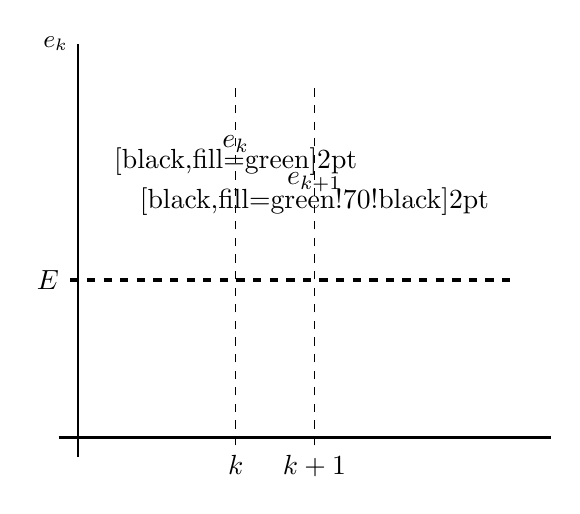
\begin{tikzpicture}
  \draw[thick,-{\seta}] (-0.25,0) -- (6,0) ;%node[above] {\small $k$};
  \draw[thick,-{\seta}] (0,-0.25) -- (0,5) node[left] {\small $e_k$};
%  \draw[] (2,0) node[below] {$k$};
  \draw[dashed] (2,-0.1) node[below] {$k$} -- (2,4.5);
%  \draw[] (3,0) node[below] {$k+1$};
  \draw[dashed] (3,-0.1) node[below] {$k+1$} -- (3,4.5);
  \draw[ultra thick,dashed] (-0.1,2) node[left] {$E$} -- (5.5,2)  ;
%
  \draw (2,3.5) node {\tikzcircle[black,fill=green]{2pt}} node[above] {$e_{k}$};
  \draw (3,3) node {\tikzcircle[black,fill=green!70!black]{2pt}} node[above] {$e_{k+1}$};
\end{tikzpicture}
\end{center}


Similarly, if $e_k < E$, we can conclude that $e_{k+1} \in [e_k,E]$:
\begin{center}
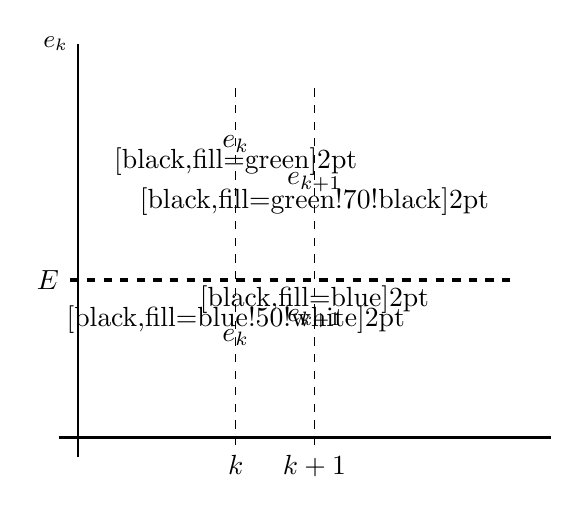
\begin{tikzpicture}
  \draw[thick,-{\seta}] (-0.25,0) -- (6,0) ;%node[above] {\small $k$};
  \draw[thick,-{\seta}] (0,-0.25) -- (0,5) node[left] {\small $e_k$};
%  \draw[] (2,0) node[below] {$k$};
  \draw[dashed] (2,-0.1) node[below] {$k$} -- (2,4.5);
%  \draw[] (3,0) node[below] {$k+1$};
  \draw[dashed] (3,-0.1) node[below] {$k+1$} -- (3,4.5);
  \draw[ultra thick,dashed] (-0.1,2) node[left] {$E$} -- (5.5,2)  ;
%
  \draw (2,3.5) node {\tikzcircle[black,fill=green]{2pt}} node[above] {$e_{k}$};
  \draw (3,3) node {\tikzcircle[black,fill=green!70!black]{2pt}} node[above] {$e_{k+1}$};
  \draw (2,1.5) node {\tikzcircle[black,fill=blue!50!white]{2pt}} node[below] {$e_{k}$};
  \draw (3,1.75) node {\tikzcircle[black,fill=blue]{2pt}} node[below] {$e_{k+1}$};
\end{tikzpicture}
\end{center}


So we can see that the sequence $e_k$ will be approaching $E$, so we can say that the \emph{equilibrium is stable}.







\hfill

\begin{center}
\textbf{\color{cyan}
Limiting behaviour of the solutions
}
\end{center}



From our previous analysis, we can see that it looks like 
$$
\lim_{k \to \infty} e_k = E.
$$

But we didn't prove this yet. It could be that the sequence converges to some other value. 

To show this, we would need to define a new sequence $x_k = e_k-E$, assume that it has the form $x_k = C r^k$ and then obtain a characteristic equation for $r$:
$$
r = 1-g-q \in (0,1),
$$
so $x_k = C r^k$ and 
$$
\lim_{k \to \infty} x_k = 0
\quad \Leftrightarrow \quad
	\lim_{k \to \infty} e_k = E.
$$

So we now know that the number of students will converge monotonically to the equilibrium.







